\subsubseccion{Ley Binomial negativa}
\label{Sssec:MP:BinomialNegativa}

Formas particulares  de esta ley aparecieron  en los a\~nos 1679  en trabajos de
Blaise  Pascal~\cite{Pas79, Hal90, DavEdw01}~\footnote{De  hecho aparece  en una
  carta  de 1654 que  mando B.  PAscal a  P. de  Fermat, publicada  mucho tiempo
  despu\'es.}     y    un    poco     m\'as    tarde     de    P.      R.     de
Montmort~\cite[p.~233-248]{Mon13}.   Esta  ley  aparece  cuando  se  repite  una
experencia binaria  exito/facasco \  con probabilidad \  $p$ \ de  exito, manera
independiente hasta el \ $r$-\'esimo  facasco ($r$ \ fijo), contendo el n\'umero
de excitos obtenidos cuando se para la experiencia.

Se denota \ $X \, \sim \, \B_-(r,p)$ \ con \ $r \in \Nset^*$, \quad $p \in [0 \;
1)$ \ y sus caracter\'isticas son las siguientes:

\begin{caracteristicas}
%
Dominio de definici\'on & $\X = \Nset$\\[2mm]
\hline
%
Par\'ametros & $r  \in \Nset^*,  \quad p \in [0  \;
1)$\\[2mm]
\hline
%
Distribuci\'on de probabilidad & \protect$\displaystyle p_X(x) = \bino{x+r-1}{x}
\, p^x (1-p)^r$\protect\\[2mm]
\hline
%
Promedio & $\displaystyle m_X = \frac{r \, p}{1-p}$\\[2mm]
\hline
%
Varianza & $\displaystyle \sigma_X^2 = \frac{r \, p}{(1-p)^2}$\\[2mm]
\hline
%
\modif{Sesgo} & $\displaystyle \gamma_X = \frac{1 + p}{\sqrt{r \, p}}$\\[2mm]
\hline
%
Curtosis por exceso & $\displaystyle \widebar{\kappa}_X = \frac{1 + 4 \, p +
p^2}{r \, p} $\\[2mm]
\hline
%
Generadora de probabilidad & $\displaystyle G_X(z) = \left( \frac{1 - p}{1 - p
\, z} \right)^r$ \ para \ $|z| < p^{-1} $\\[2mm]
\hline
%
Generadora de momentos & $\displaystyle M_X(u) = \left( \frac{1 - p}{1 - p \,
e^u } \right)^r$ \ para \ $\real{u} < - \ln p$\\[2mm]
\hline
%
Funci\'on caracter\'istica & $\displaystyle \Phi_X(\omega) = \left( \frac{1 -
p}{1 - p \, e^{i \omega} } \right)^r$
\end{caracteristicas}

% Momentos & $ \Esp\left[ X^k \right] = ??\\[2mm]
% Momento factorial & $\Esp\left[ (X)_k \right] = 
% \frac{(r+k-1)!}{(r-1)!} \left( \frac{p}{1-p} \right)^k$\\[2mm]
% Modo $\left\lfloor (n+1) p \right\rfloor$
% Mediana $\left\lfloor n p \right\rfloor$ o $\left\lceil n p \right\rceil
% CDF	$I_{1-p}(n-k,k+1)$ regularized incomplete beta function

Su masa  de probabilidad  y funci\'on de  repartici\'on son representadas  en la
figura Fig.~\ref{Fig:MP:BinomialNegativa}.
%
\begin{figure}[h!]
\begin{center} 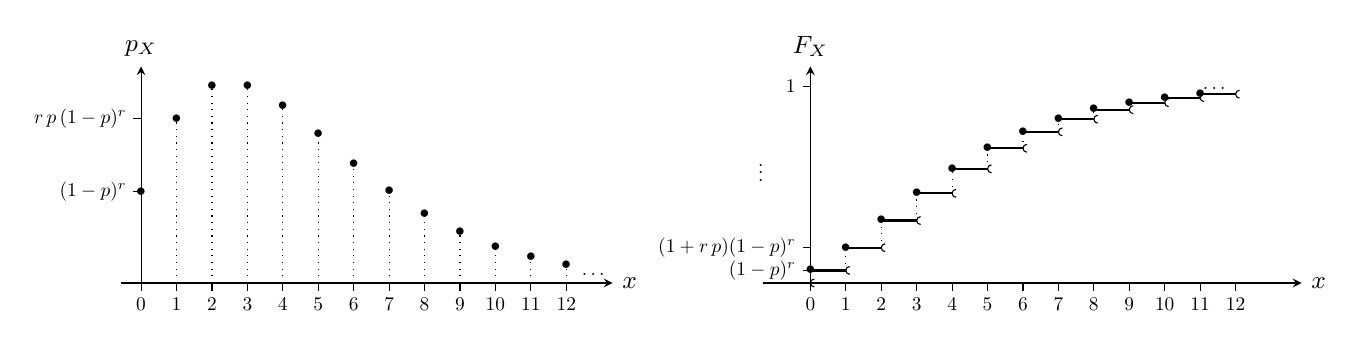
\begin{tikzpicture}%[scale=.9]
\shorthandoff{>}
%
\pgfmathsetmacro{\sx}{.45};% x-scaling
\pgfmathsetmacro{\r}{.05};% radius arc non continuity F_X
\pgfmathsetmacro{\p}{3/5};% probabilidad p de suceso
\pgfmathsetmacro{\rp}{3};% numero r de fracascos
\pgfmathsetmacro{\n}{12};% numero maximo a dibujar
\pgfmathsetmacro{\q}{max(floor((\rp-1)*\p/(1-\p)),0)};% modo de la binomial negativa
\pgfmathsetmacro{\m}{factorial(\q+\rp-1)*((1-\p)^\rp)*(\p^\q)/factorial(\rp-1)/factorial(\q)};
%{factorial(\n)/factorial(\q)/factorial(\n-\q)*(\p^\q)*((1-\p)^(\n-\q))};% maximo de la binomial
% masa
\begin{scope}
%
\pgfmathsetmacro{\sy}{2.5/\m};% y-scaling 
\draw[>=stealth,->] (-.25,0)--({\sx*(\n+.75)+.25},0) node[right]{\small $x$};
\draw[>=stealth,->] (0,-.1)--(0,{\sy*\m+.25}) node[above]{\small $p_X$};
%
\pgfmathsetmacro{\b}{(1-\p)^\rp};% coeficiente binomial por la probabilidad
%
\foreach \k in {0,...,\n} {
\draw ({\k*\sx},0)--({\k*\sx},-.1) node[below,scale=.7]{$\k$};
\draw[dotted] ({\k*\sx},0)--({\k*\sx},{\sy*\b}) node[scale=.7]{$\bullet$};
%
\pgfmathsetmacro{\bl}{\b*\p*(\k+\rp)/(\k+1)};\global\let\b\bl;% proba actualizada
}
\draw ({(\n+.25)*\sx},{\sy*\b*(\n+1)/\p/(\n+\rp)/2}) node[right,scale=.7]{\ldots};
\draw (0,{((1-\p)^\rp)*\sy})--(-.1,{((1-\p)^\rp)*\sy}) node[left,scale=.7]{$(1-p)^r$};
\draw (0,{\rp*\p*((1-\p)^\rp)*\sy})--(-.1,{\rp*\p*((1-\p)^\rp)*\sy}) node[left,scale=.7]{$r \, p \, (1-p)^r$};
%\draw (0,{(\rp*\p*((1-\p)^\rp)+\m)/2*\sy}) node[scale=.7]{$r \, p \, (1-p)^r$};
%
\end{scope}
%
%
% reparticion
\begin{scope}[xshift=8.5cm]
%
\pgfmathsetmacro{\sy}{2.5};% y-scaling 
%
\draw[>=stealth,->] (-.6,0)--({\sx*(\n+.75)+.5},0) node[right]{\small $x$};
\draw[>=stealth,->] (0,-.1)--(0,{\sy+.25}) node[above]{\small $F_X$};
%
\pgfmathsetmacro{\b}{(1-\p)^\rp};% coeficiente binomial por la probabilidad
\pgfmathsetmacro{\c}{(1-\p)^\rp};% cumulativa binomial por la probabilidad
%
% cumulativa x < 0
\draw (0,0)--(0,-.1) node[below,scale=.7]{$0$};
\draw[thick] (-.5,0)--(0,0);
\draw (\r,\r) arc (90:270:\r);
%
% cumulativa x de 0 a n-1
\foreach \k in {1,...,\n} {
\draw ({\k*\sx},0)--({\k*\sx},-.1) node[below,scale=.7]{$\k$};
\draw[thick]({(\k-1)*\sx},{\sy*\c}) node[scale=.7]{$\bullet$}--({\k*\sx},{\sy*\c});
\draw ({\k*\sx+\r},{\sy*\c+\r}) arc (90:270:\r);
\draw[dotted] ({(\k-1)*\sx},{(\c-\b)*\sy})--({(\k-1)*\sx},{\c*\sy});
%
\pgfmathsetmacro{\bl}{\b*\p*(\k+\rp-1)/\k};\global\let\b\bl;% proba actualizada
\pgfmathsetmacro{\cl}{\c+\b};\global\let\c\cl;% cumulativa actualizada
}
%
\draw ({\n*\sx},{\sy*(\c+1)/2}) node[left,scale=.7]{\ldots};
\draw (0,{((1-\p)^\rp)*\sy})--(-.1,{((1-\p)^\rp)*\sy}) node[left,scale=.7]{$(1-p)^r$};
\draw (0,{(1+\rp*\p)*((1-\p)^\rp)*\sy})--(-.1,{(1+\rp*\p)*((1-\p)^\rp)*\sy}) node[left,scale=.7]{$(1+r \, p) (1-p)^r$};
\draw (-.75,{((1+\rp*\p)*((1-\p)^\rp)+1)/2*\sy}) node[right,scale=.7]{$\vdots$};
\draw (0,\sy)--(-.1,\sy) node[left,scale=.7]{$1$};
\end{scope}
%
\end{tikzpicture} \end{center}
%
\leyenda{Ilustraci\'on de  una distribuci\'on de  probabilidad binomial negativa
  (a), y  la funci\'on  de repartici\'on  asociada (b), con  $r =  3, \quad  p =
  \frac35$.}
\label{Fig:MP:BinomialNegativa}
\end{figure}
\SZ{Otros ilustraciones para otros $r, p$?}

Recordar que esta ley aparece cuando se repite una experencia binaria \ $X_i \in
\{ 0 \;  1 \}, i = 1, \ldots$  \ con \ $P(X_i=1) = p$  \ de manera independiente
($X_i$ independientes) hasta que \ $r$ \ variables valen 0, con \ $r$ \ fijo. El
n\'umero  de  excito  \ $X$  \  sigue  una  ley  \  $\B_-(r,p)$ (el  calculo  es
directo). Dicho de  otra manera, $X =  \sum_{i=1}^N X_i$ \ con \  $N$ \ variable
aleatoria tal que $X_N = 0$ \ y \ $r = \sum_{i=1}^N (1-X_i)$: condicionalmente a
\ $N$, la variable  \modif{\ $X$ } \ es binomial de  par\'ametro $p$\modif{, \ie \
  $P(X=x|N=n) = \bino{n}{x}  p^x (1-p)^{n-x}$}.  Se puede ver que \  $P(N = n) =
\bino{n}{r-1} (1-p)^r  p^{n-r}$ \ y la  ley de la binomial  negativa se recupera
\modif{a        trav\'es        del        teorema        de        probabilidad
  total~\ref{Teo:MP:ProbaTotalDiscreto}    o   tambi\'en,}   a    trav\'es   del
teorema~\ref{Teo:MP:SumaAleatoriaGeneradoraProbabilidad}.
%
% Blaise PAscal - Polya caso r real

Esta distribuci\'on se  generaliza para \ $r \in \Rset_+^*$ \  pero se pierde la
interpretaci\'on que v\'imos en el p\'arafo anterior.

Nota: cuando \ $p = 0$ \ la variable es cierta \ $X = r$.